\chapter{Execuções para o \emph{fitness} $f_i = e^{-\lambda||\nabla\rho||^2}$}

\begin{figure}[htbp]
\centering
  \begin{tabular}{@{}cc@{}}
    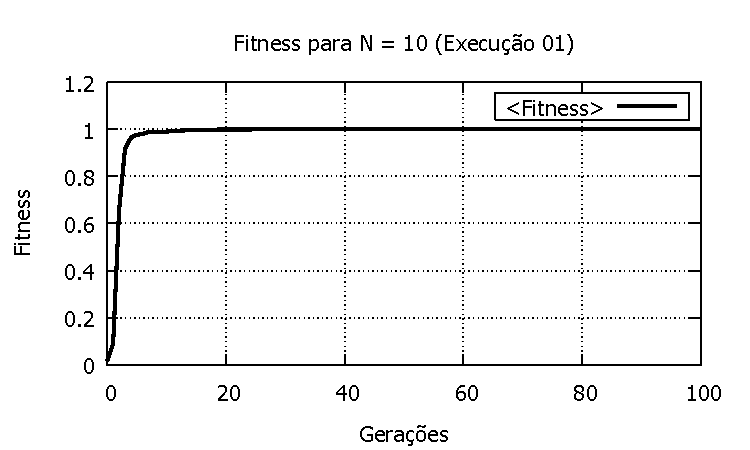
\includegraphics[width=.45\textwidth]{figs/resultados/fitnessGrad/N10_01_fitness.pdf} &
    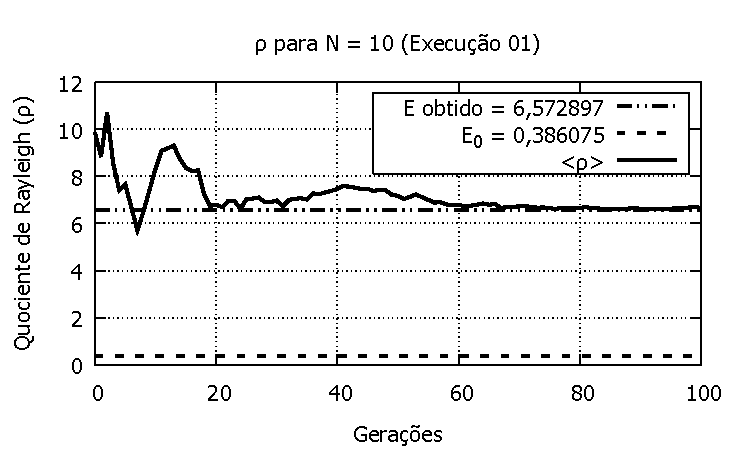
\includegraphics[width=.45\textwidth]{figs/resultados/fitnessGrad/N10_01_rho.pdf}   \\
		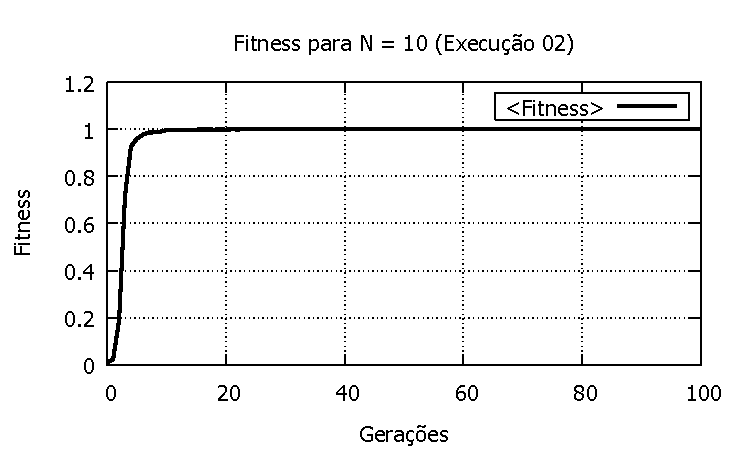
\includegraphics[width=.45\textwidth]{figs/resultados/fitnessGrad/N10_02_fitness.pdf} &
    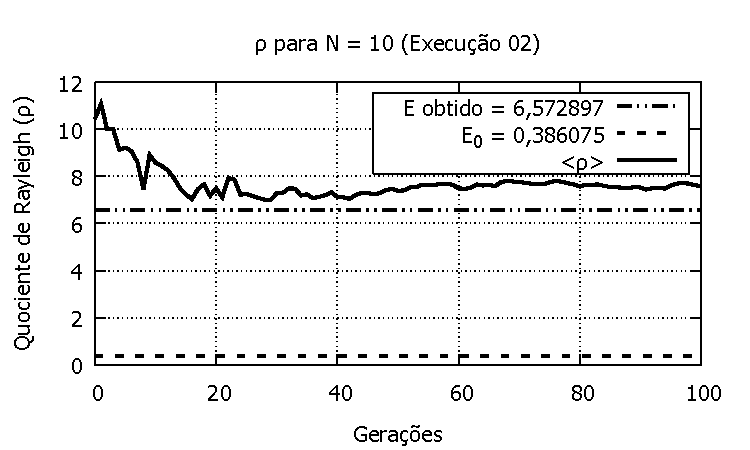
\includegraphics[width=.45\textwidth]{figs/resultados/fitnessGrad/N10_02_rho.pdf}   \\
		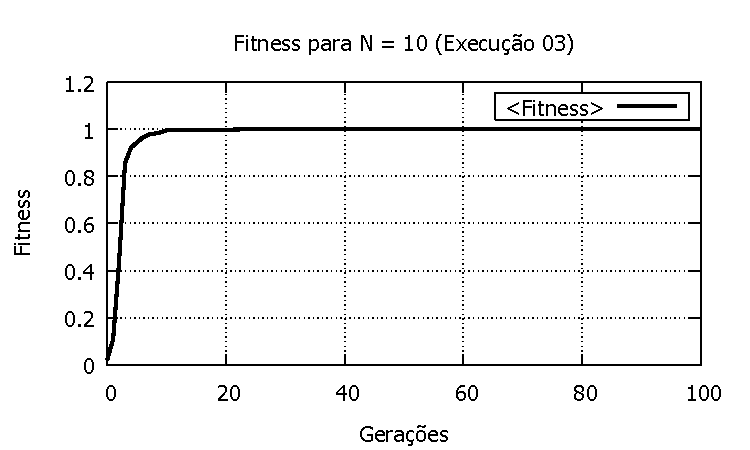
\includegraphics[width=.45\textwidth]{figs/resultados/fitnessGrad/N10_03_fitness.pdf} &
    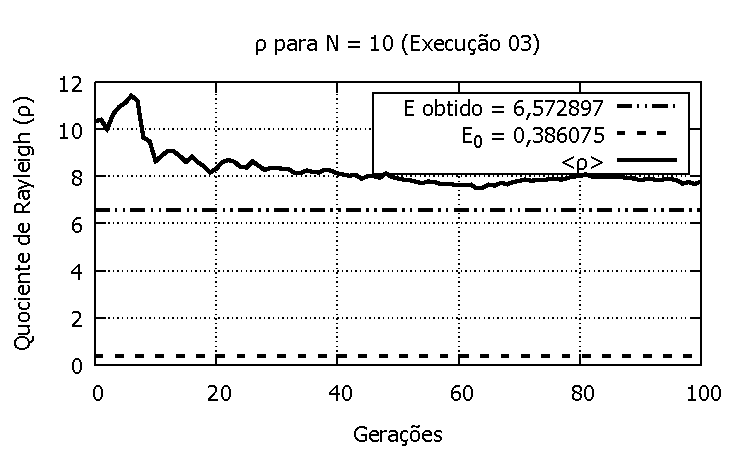
\includegraphics[width=.45\textwidth]{figs/resultados/fitnessGrad/N10_03_rho.pdf}   \\
		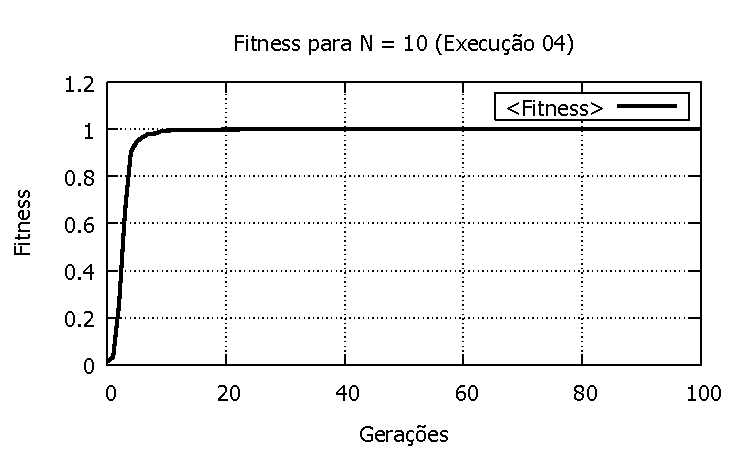
\includegraphics[width=.45\textwidth]{figs/resultados/fitnessGrad/N10_04_fitness.pdf} &
    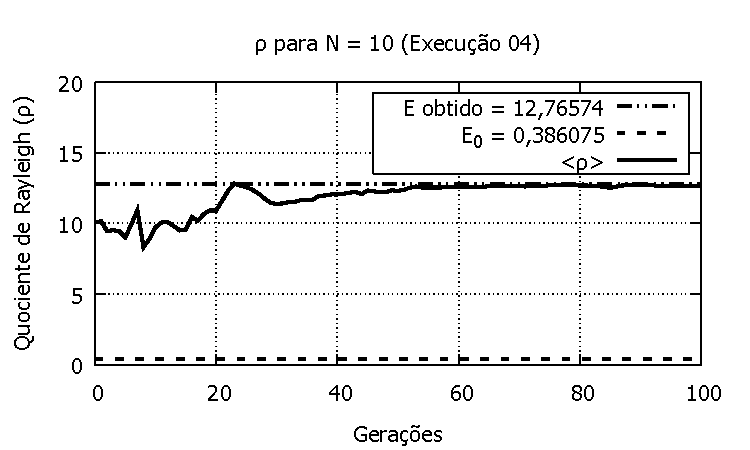
\includegraphics[width=.45\textwidth]{figs/resultados/fitnessGrad/N10_04_rho.pdf}   \\
		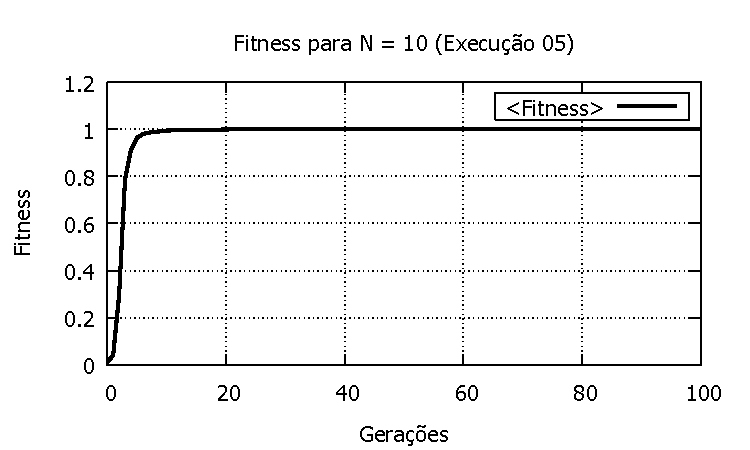
\includegraphics[width=.45\textwidth]{figs/resultados/fitnessGrad/N10_05_fitness.pdf} &
    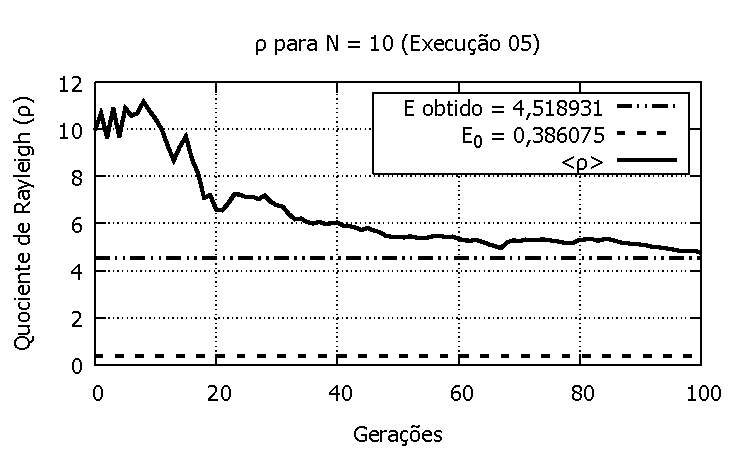
\includegraphics[width=.45\textwidth]{figs/resultados/fitnessGrad/N10_05_rho.pdf}
    %\multicolumn{2}{c}{\includegraphics[width=.23\textwidth]{example-image-a}}
  \end{tabular}
  \caption{Execuções N = 10.}
	\label{fig:execucoes_N10}
\end{figure}

\begin{figure}[htbp]
\centering
  \begin{tabular}{@{}cc@{}}
    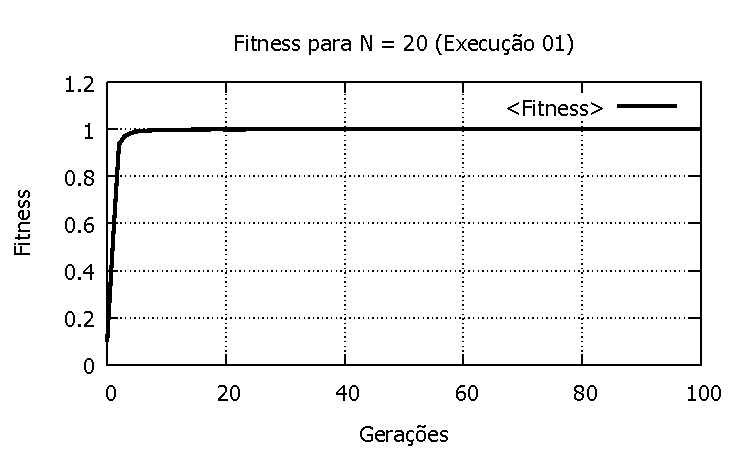
\includegraphics[width=.45\textwidth]{figs/resultados/fitnessGrad/N20_01_fitness.pdf} &
    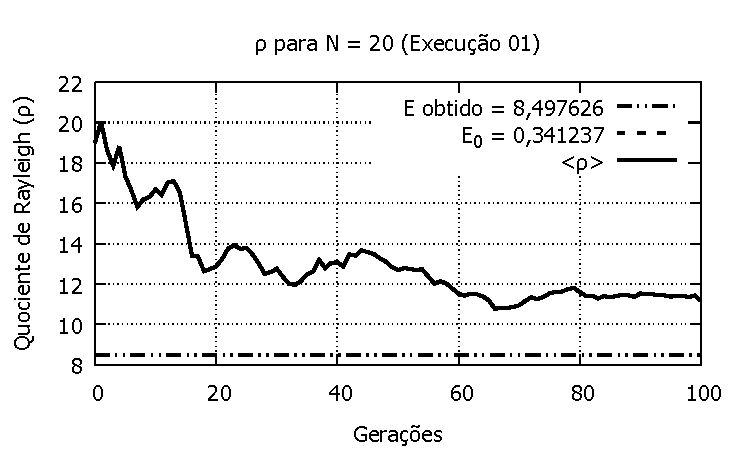
\includegraphics[width=.45\textwidth]{figs/resultados/fitnessGrad/N20_01_rho.pdf}   \\
		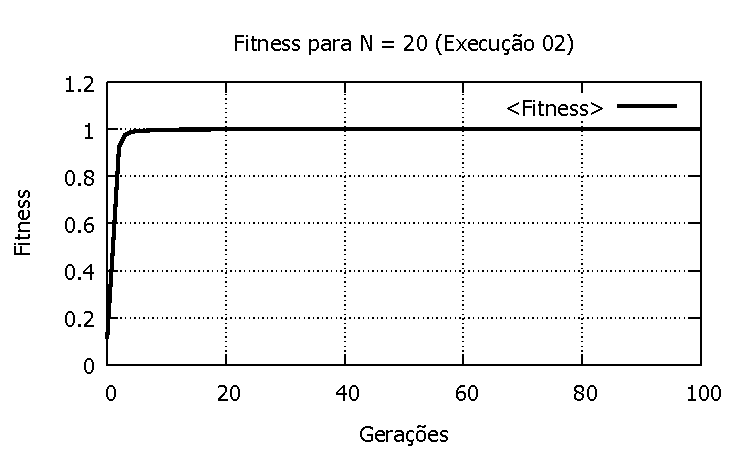
\includegraphics[width=.45\textwidth]{figs/resultados/fitnessGrad/N20_02_fitness.pdf} &
    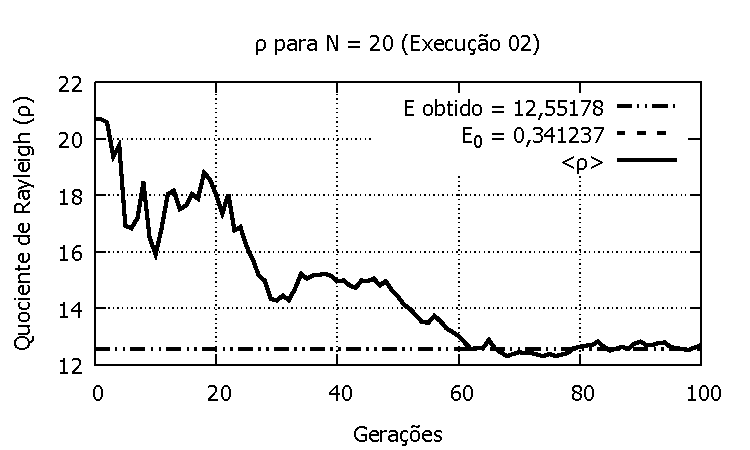
\includegraphics[width=.45\textwidth]{figs/resultados/fitnessGrad/N20_02_rho.pdf}   \\
		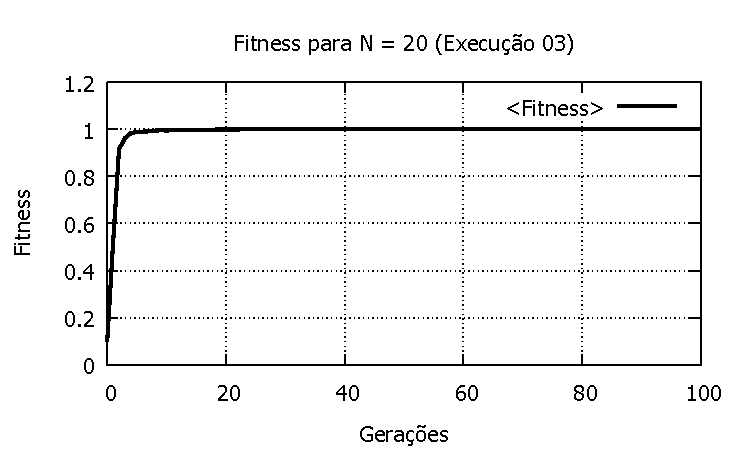
\includegraphics[width=.45\textwidth]{figs/resultados/fitnessGrad/N20_03_fitness.pdf} &
    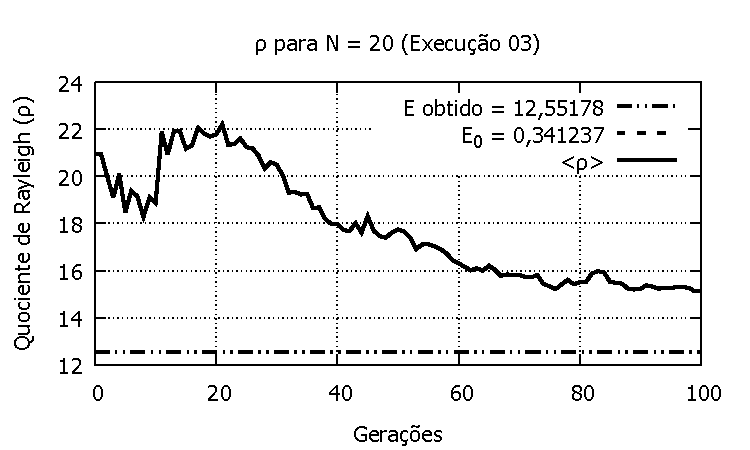
\includegraphics[width=.45\textwidth]{figs/resultados/fitnessGrad/N20_03_rho.pdf}   \\
		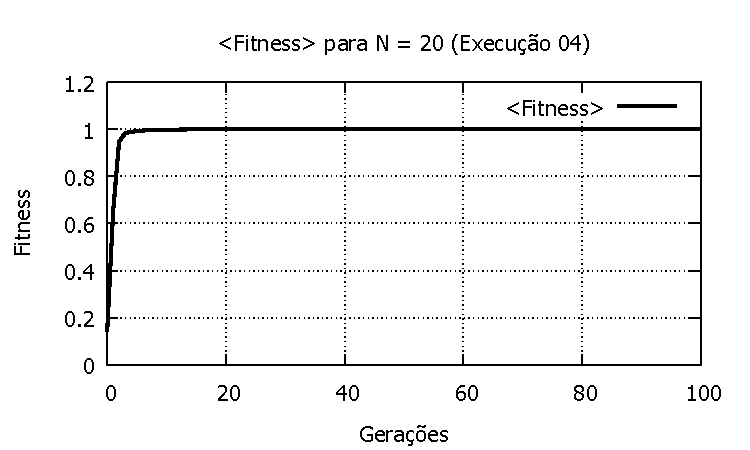
\includegraphics[width=.45\textwidth]{figs/resultados/fitnessGrad/N20_04_fitness.pdf} &
    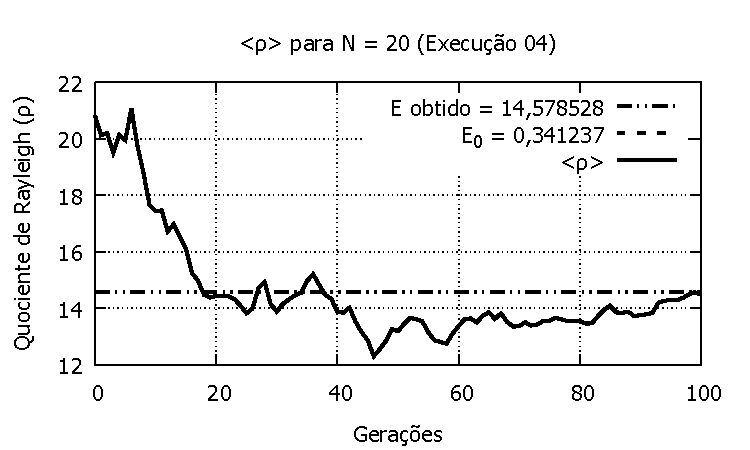
\includegraphics[width=.45\textwidth]{figs/resultados/fitnessGrad/N20_04_rho.pdf}   \\
		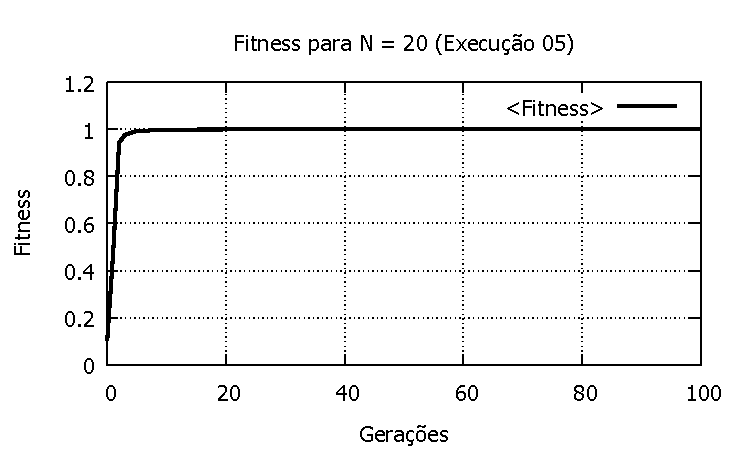
\includegraphics[width=.45\textwidth]{figs/resultados/fitnessGrad/N20_05_fitness.pdf} &
    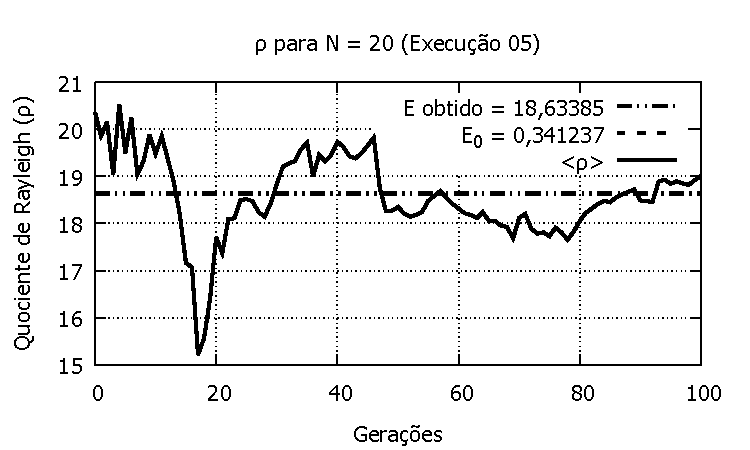
\includegraphics[width=.45\textwidth]{figs/resultados/fitnessGrad/N20_05_rho.pdf}
    %\multicolumn{2}{c}{\includegraphics[width=.23\textwidth]{example-image-a}}
  \end{tabular}
  \caption{Execuções N = 20.}
	\label{fig:execucoes_N20}
\end{figure}

\begin{figure}[htbp]
\centering
  \begin{tabular}{@{}cc@{}}
    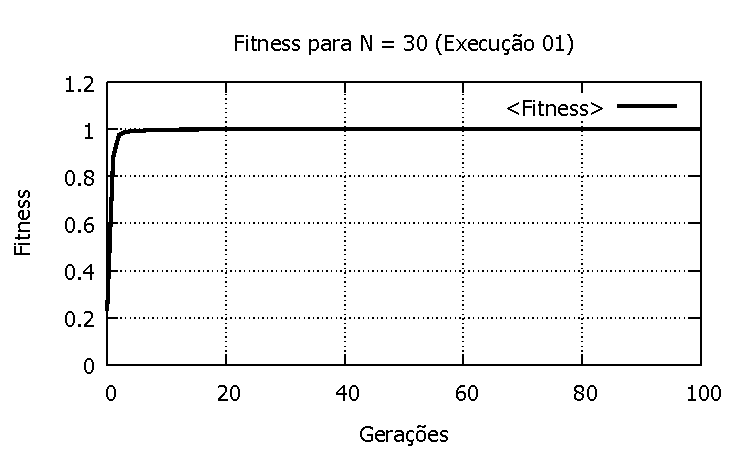
\includegraphics[width=.45\textwidth]{figs/resultados/fitnessGrad/N30_01_fitness.pdf} &
    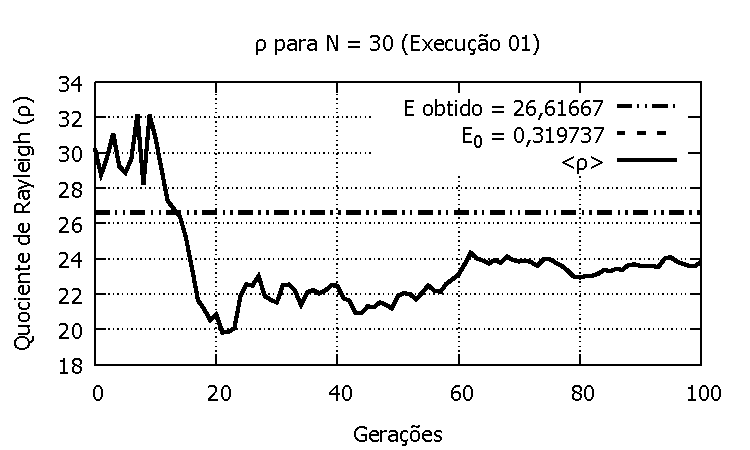
\includegraphics[width=.45\textwidth]{figs/resultados/fitnessGrad/N30_01_rho.pdf}   \\
		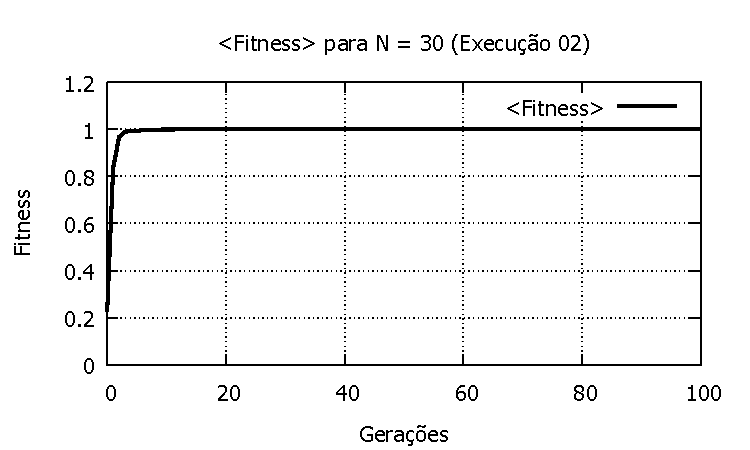
\includegraphics[width=.45\textwidth]{figs/resultados/fitnessGrad/N30_02_fitness.pdf} &
    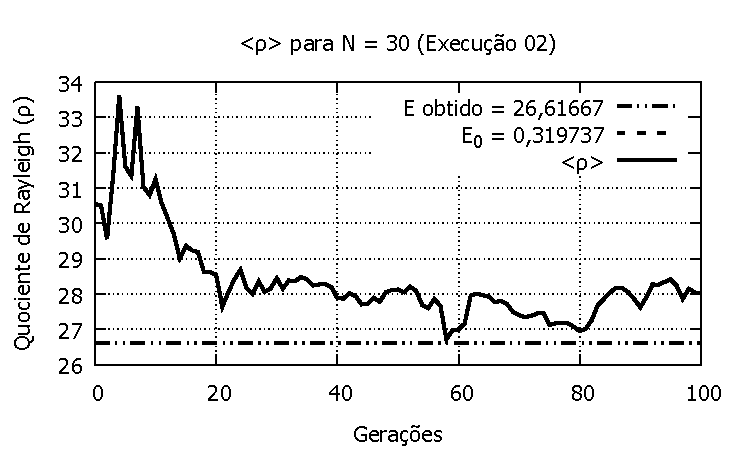
\includegraphics[width=.45\textwidth]{figs/resultados/fitnessGrad/N30_02_rho.pdf}   \\
		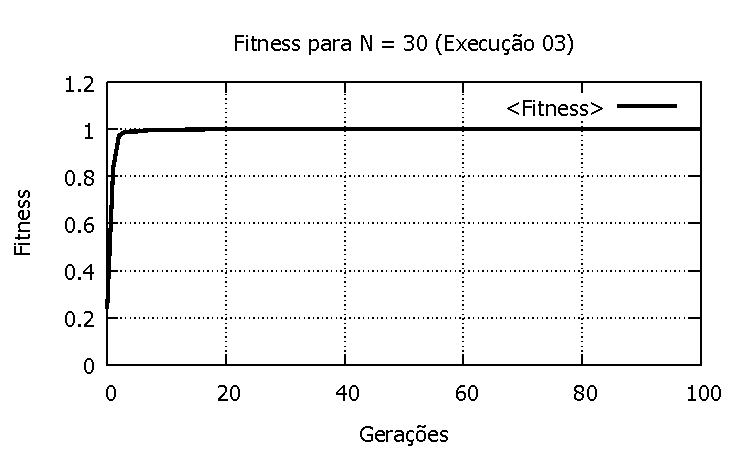
\includegraphics[width=.45\textwidth]{figs/resultados/fitnessGrad/N30_03_fitness.pdf} &
    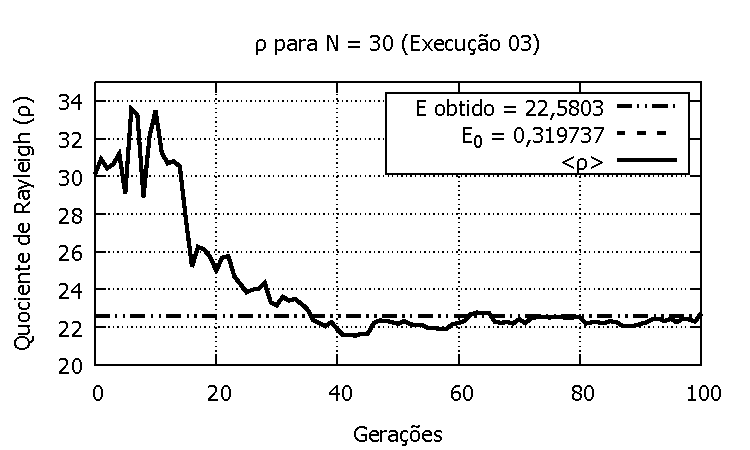
\includegraphics[width=.45\textwidth]{figs/resultados/fitnessGrad/N30_03_rho.pdf}   \\
		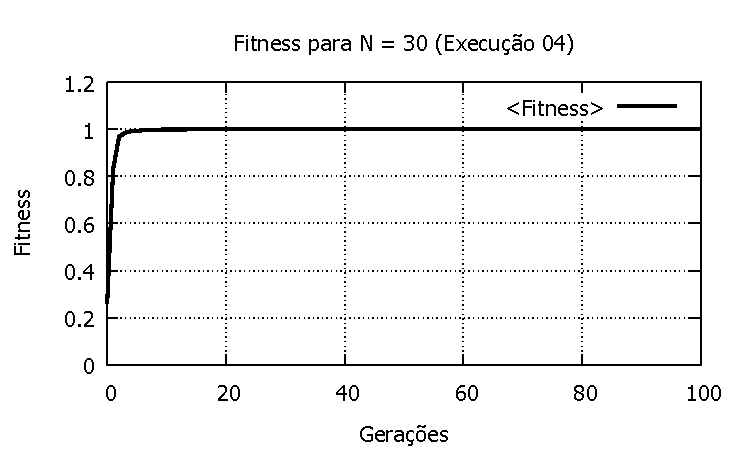
\includegraphics[width=.45\textwidth]{figs/resultados/fitnessGrad/N30_04_fitness.pdf} &
    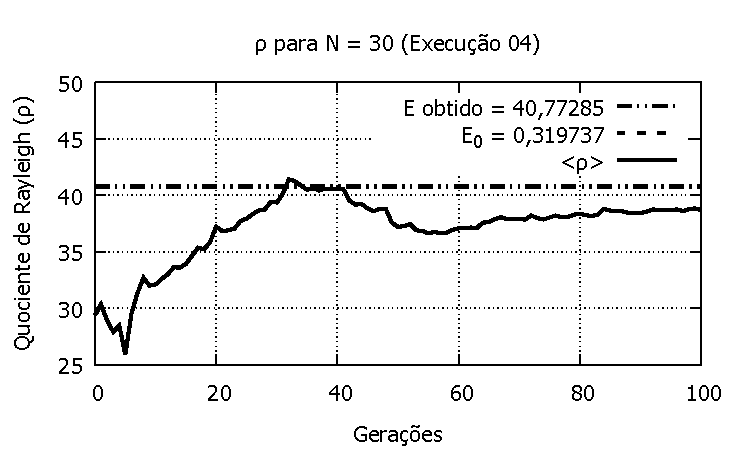
\includegraphics[width=.45\textwidth]{figs/resultados/fitnessGrad/N30_04_rho.pdf}   \\
		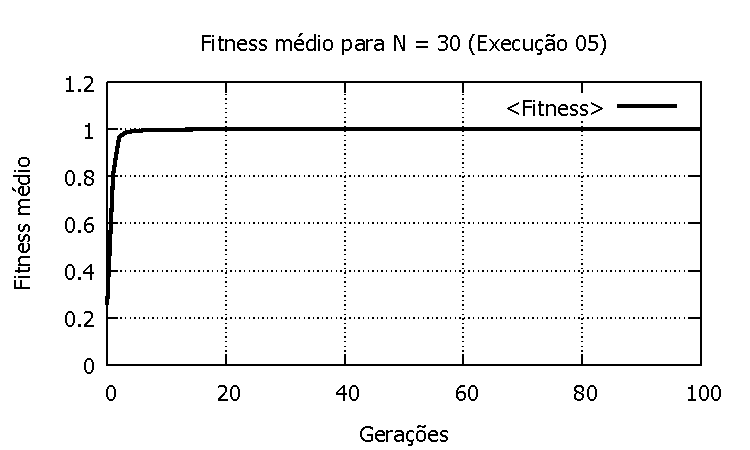
\includegraphics[width=.45\textwidth]{figs/resultados/fitnessGrad/N30_05_fitness.pdf} &
    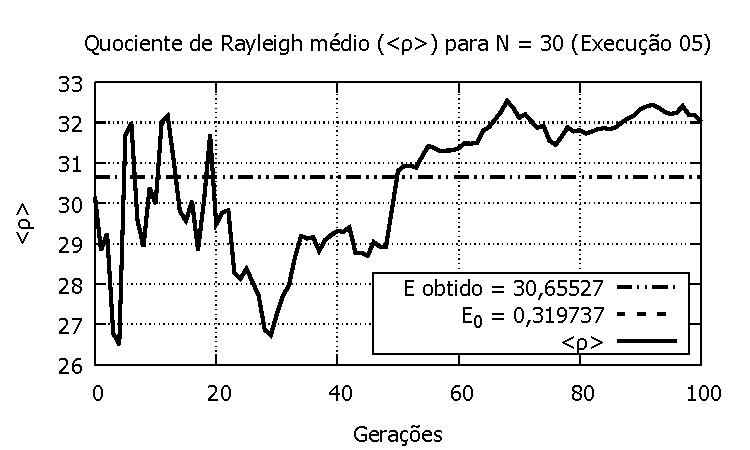
\includegraphics[width=.45\textwidth]{figs/resultados/fitnessGrad/N30_05_rho.pdf}
    %\multicolumn{2}{c}{\includegraphics[width=.23\textwidth]{example-image-a}}
  \end{tabular}
  \caption{Execuções N = 30.}
	\label{fig:execucoes_N30}
\end{figure}

\begin{figure}[htbp]
\centering
  \begin{tabular}{@{}cc@{}}
    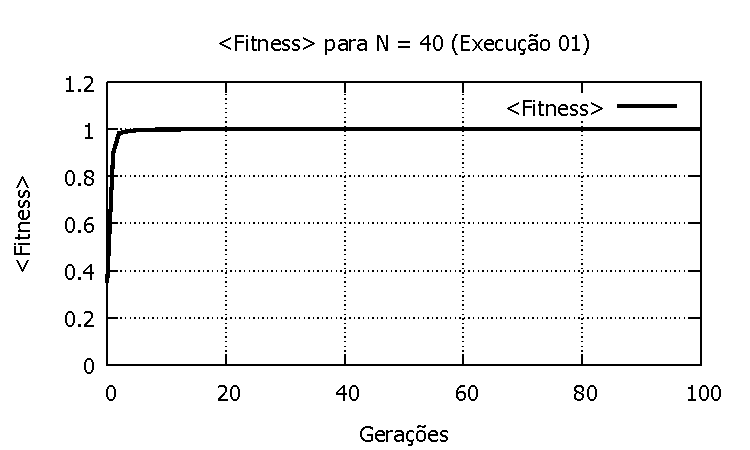
\includegraphics[width=.45\textwidth]{figs/resultados/fitnessGrad/N40_01_fitness.pdf} &
    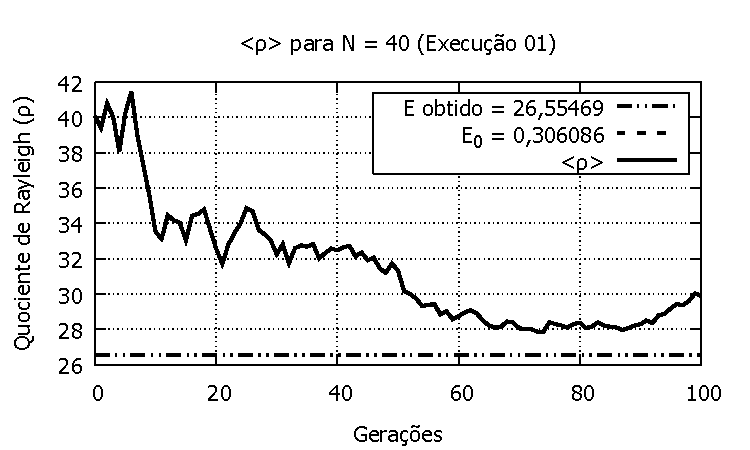
\includegraphics[width=.45\textwidth]{figs/resultados/fitnessGrad/N40_01_rho.pdf}   \\
		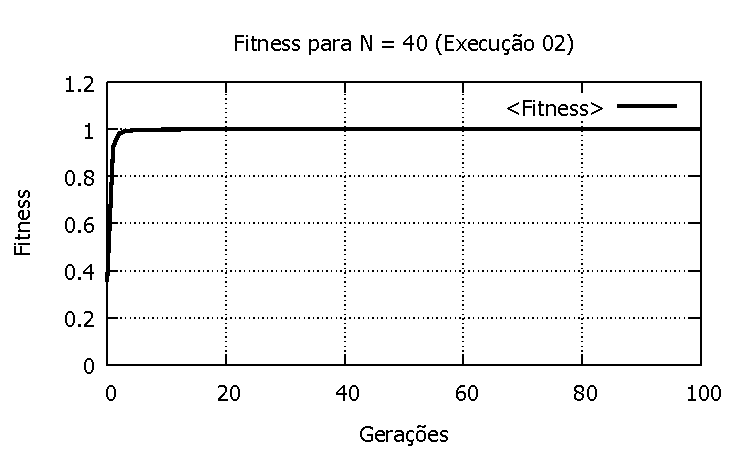
\includegraphics[width=.45\textwidth]{figs/resultados/fitnessGrad/N40_02_fitness.pdf} &
    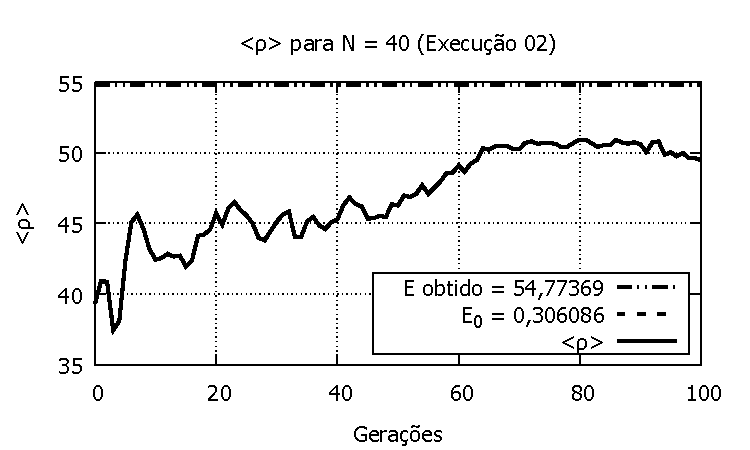
\includegraphics[width=.45\textwidth]{figs/resultados/fitnessGrad/N40_02_rho.pdf}   \\
		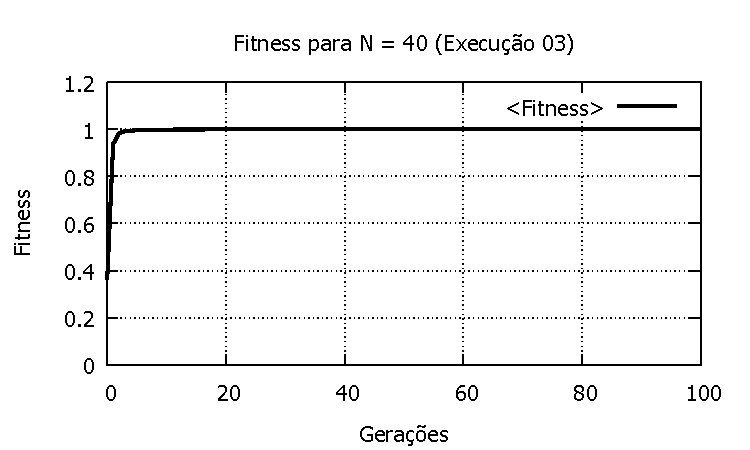
\includegraphics[width=.45\textwidth]{figs/resultados/fitnessGrad/N40_03_fitness.pdf} &
    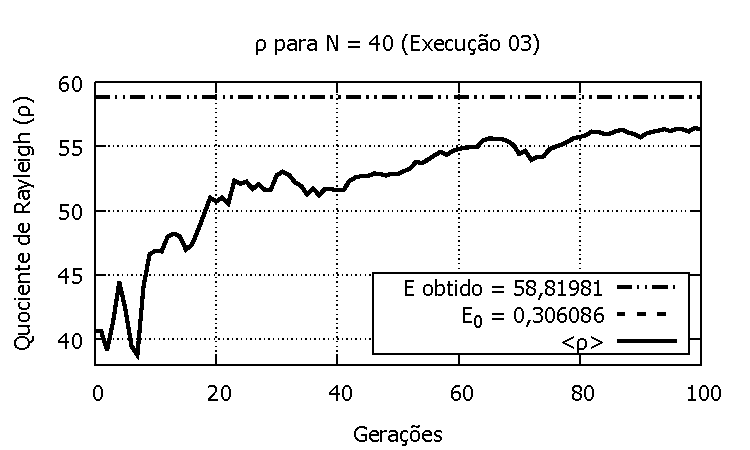
\includegraphics[width=.45\textwidth]{figs/resultados/fitnessGrad/N40_03_rho.pdf}   \\
		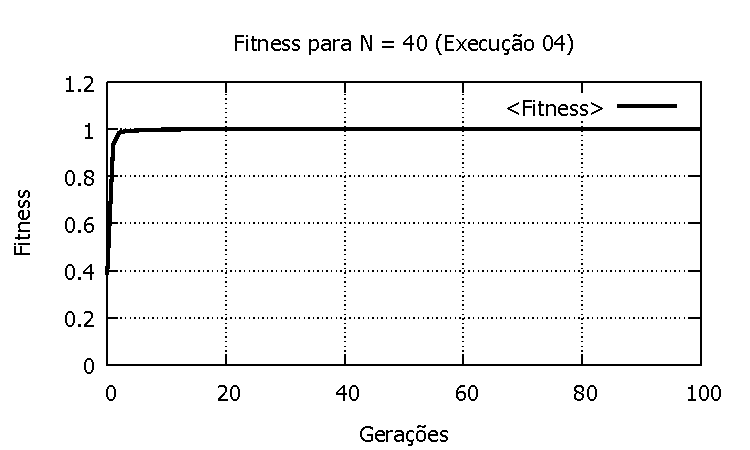
\includegraphics[width=.45\textwidth]{figs/resultados/fitnessGrad/N40_04_fitness.pdf} &
    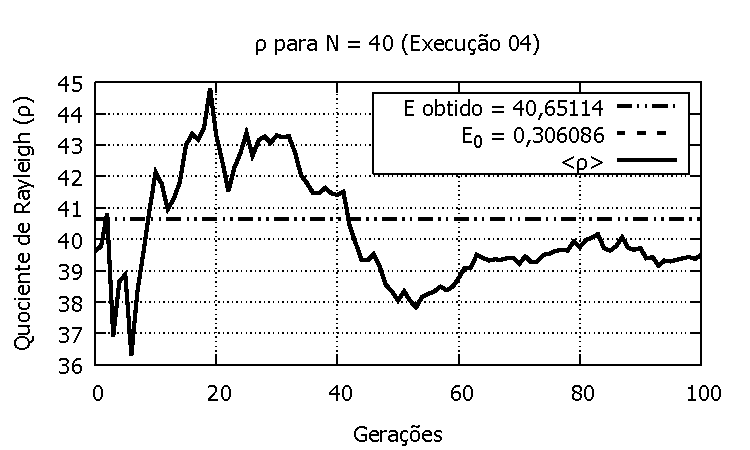
\includegraphics[width=.45\textwidth]{figs/resultados/fitnessGrad/N40_04_rho.pdf}   \\
		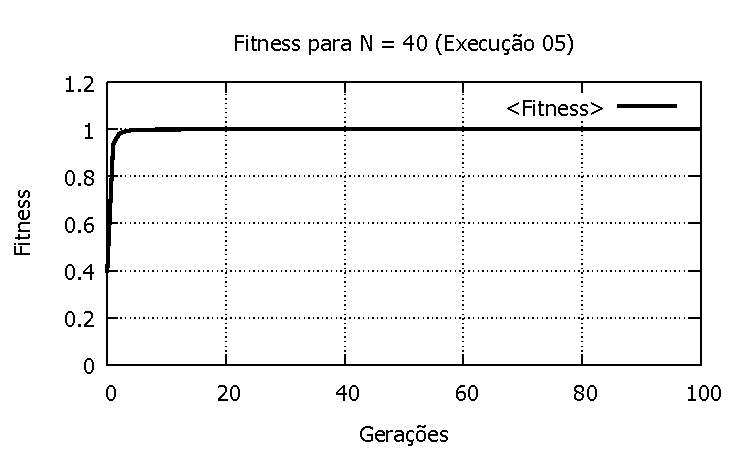
\includegraphics[width=.45\textwidth]{figs/resultados/fitnessGrad/N40_05_fitness.pdf} &
    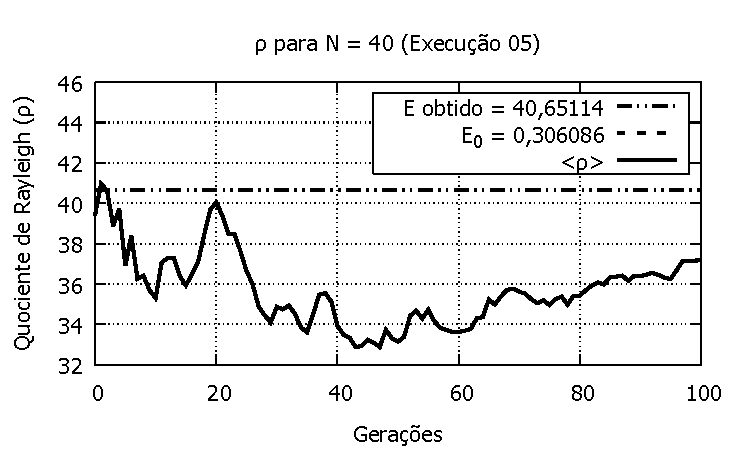
\includegraphics[width=.45\textwidth]{figs/resultados/fitnessGrad/N40_05_rho.pdf}
    %\multicolumn{2}{c}{\includegraphics[width=.23\textwidth]{example-image-a}}
  \end{tabular}
  \caption{Execuções N = 40.}
	\label{fig:execucoes_N40}
\end{figure}